\chapter{Articles}

\section{Abstract}

The most interesting researches and probably the ones that will be used are :
\begin{itemize}
	\item \citeref{res1}
	\item \citeref{res2}
	\item \citeref{res4}
	\item \citeref{res5}
	\item \citeref{res6}
\end{itemize}

\section{MRI-based DL/ML}

\newpage
\subsection{\href{https://www.sciencedirect.com/science/article/pii/S187887502032698X}{[NGUYEN2021E1112] Convolutional Neural Networks for Pediatric Refractory Epilepsy Classification Using Resting-State Functional Magnetic Resonance Imaging (May 2021) }}
\label{res1}


Study made to evaluate the performance of CNN in "the classification of patients with paediatric epilepsy from healthy control"

To modify CNNs, some parameters were manually changed, such as: 3 hyperparameters, learning rate, dropout rate and regularization, and number of epoch.

To evaluate them ($\sim$4000 models), the model with the highest sensitivity was kept.

Could be used to test other programs.

\subsubsection{Methods}

Full explanations of each step in the paper, figure summing up here: \citeref{fig:res1}

\begin{figure}[htbp]
	\centering
	\includegraphics[width=\textwidth]{"CNN_explanation.jpg"}
	\caption{Linked to this research: \citeref{res1}}%
	\label{fig:res1}
\end{figure}

\subsubsection{Results}

Results here: \citeref{tab:res1}

\begin{table}[htbp]
	\centering
	\fbox{
	\begin{tabular}{l c}
		n & 322 \\
		patients & 63 \\
		controls & 259 \\
		train ratio & 0.6 \\
		validate ratio & 0.2 \\
		test ratio & 0.2 \\
	\end{tabular}
}
	\caption{Benchmark}

	\fbox{
	\begin{tabular}{l c}
		Sensitivity & 85\% \\
		Specificity & 71\% \\
		F1 score & 0.56 \\
	\end{tabular}
}
	\caption{Results of \citeref{res1}}%

	\fbox{
		\begin{tabular}{l c}
			Dropout rate & 50\% \\
			Learning rate & $1e-4$ \\
			Epoch & 181 \\
		\end{tabular}
	}
	\caption{Best model parameter values}
	\label{tab:res1}
\end{table}

\newpage
\subsection{\href{https://academic.oup.com/brain/article/145/11/3859/6659752?login=true}{[AWAC224101093] Interpretable surface-based detection of focal cortical dysplasias: a Multi-centre Epilepsy Lesion Detection study (August 2022) }}
\label{res2}

Code via GitHub here: \citeref{code:res2}

\subsubsection{Methods}

Explanation here: \citeref{fig:meld_explanation}

Cohort splitting: 50-50 and 10-fold cross-validation

From MRI images, brain is reconstructed via \emph{FreeSurfer} library. It then consists in a lot of vertices and edges.
These are analysed by the model to declare lesioned vertices.

\begin{figure}[htbp]
	\centering
	\includegraphics[width=\textwidth]{"meld_method.pdf"}
	\caption{Linked to this research: \citeref{res2}}%
	\label{fig:meld_explanation}
\end{figure}

\subsubsection{Results}

\begin{table}[htbp]
	\centering
	\fbox{
	\begin{tabular}{l c}
		n & 1015 \\
		patients & 618 \\
		controls & 397 \\
		train ratio & 0.5 \\
		test ratio & 0.5 \\
	\end{tabular}
}
	\caption{Benchmark}

	\fbox{
	\begin{tabular}{l c}
		Sensitivity & 59\% \\
		Specificity & 54\% \\
	\end{tabular}
}
	\caption{Results}
\end{table}

\newpage
\subsection{\href{https://www.sciencedirect.com/science/article/pii/S1746809419301211\#sec0010}{[BIJAYDEV2019218] Automatic detection and localization of Focal Cortical Dysplasia lesions in MRI using fully convolutional neural network (2019)}}
\label{res4}

Some maths for the loss function, clear explanation on how it works.
Lots of information about the whole setup, procedure, method, neural network\dots

MRI images are taken in the sagittal plane

\subsubsection{Preprocessing}

\begin{figure}[htbp]
	\centering
	\includegraphics[width=\textwidth]{"MRI_example.jpg"}
	\caption{From research: \citeref{res4}}
	\label{fig:res4:1}
\end{figure}

\begin{figure}[htbp]
	\centering
	\includegraphics[width=\textwidth]{"MRI_example_2.jpg"}
	\caption{From research: \citeref{res4}}
	\label{fig:res4:2}
\end{figure}

\subsubsection{Method}

Fully connected convolutional network is used in order to keep the size of the image and to result into an image where each pixel corresponds to a probability of being lesioned.

Loss function: loss = Binary Cross-Entropy + Dice Loss

5-fold cross-validation where one patient frames would stay in the same fold to avoid biases

\begin{table}
	\centering
	\fbox{
	\begin{tabular}{l c}
		epochs & 100 \\
		learning rate & 0.4 \\
	\end{tabular}
}
	\caption{Interesting values of \citeref{res4}}
\end{table}

\begin{figure}[htbp]
	\centering
	\includegraphics[width=\textwidth]{"CNN_explanation_2.jpg"}
	\caption{From research: \citeref{res4}}
	\label{fig:res4:3}
\end{figure}

\subsubsection{Results}

Here: \citeref{tab:res4}

\begin{table}[htbp]
	\centering
	\fbox{
	\begin{tabular}{l c}
		subjects & 43 \\
		n (MRI frames) & 8849 \\
		patients & 1431 \\
		controls & 7418 \\
		train ratio & 0.65 \\
		test ratio & 0.18 \\
		validation ratio & 0.17 \\
	\end{tabular}
}
	\caption{Benchmark}

	\fbox{
	\begin{tabular}{l c}
		Recall & 40.10 \% \\
		Precision & 80.69 \% \\
		Dice-coefficient & 52.47 \\
	\end{tabular}
}
	\caption{Results from: \citeref{res4}}
	\label{tab:res4}
\end{table}

\newpage
\subsection{\href{https://link.springer.com/chapter/10.1007/978-3-030-00931-1_56}{[10.1007/978-3-030-00931-1-56] Deep Convolutional Networks for Automated Detection of Epileptogenic Brain Malformations (2018) }}
\label{res5}

This one uses "two identical CNN which weights are optimized independently".

MRI images used are taken in the transverse plane

\subsubsection{Method}

5-fold corss-validation

\begin{figure}[htbp]
	\centering
	\includegraphics[width=\textwidth]{"two_CNN_explanation.png"}
	\caption{Top panel: Convolutional network architecture (CNNx) for two-label (lesional vs. non-lesional) classification. Bottom panel: Training and testing schema using two-stage CNNx cascade (CNN1/CNN2). From research in \citeref{res5}}
\end{figure}

\subsubsection{Results}

Here: \citeref{tab:res5}

\begin{table}[htbp]
	\centering
	\fbox{
		\begin{tabular}{l c}
			not clear & \\
			n &  \\
			patients & 107 \\
			controls & 101 \\
			train ratio & 0.75 \\
			test ratio & 0.25 \\
		\end{tabular}
	}
	\caption{Benchmark}

	\fbox{
		\begin{tabular}{l c}
			Sensitivity & 87\% \\
			Specificity & 95\% \\
		\end{tabular}
	}
	\caption{Results from \citeref{res5}}
	\label{tab:res5}
\end{table}

\newpage
\subsection{\href{https://www.sciencedirect.com/science/article/pii/S0920121121002709\#sec0010}{[ITO2021106815] Deep learning-based diagnosis of temporal lobe epilepsy associated with hippocampal sclerosis: An MRI study (2021) }}
\label{res6}

Not to actually detect FCD but works same.

Lots of details on patient and control image acquisitions.
Also on the detail of MRIs

MRI images are taken in the transverse plane

\subsubsection{Method}

5-fold cross-validation, 
use of CNN, 
data augmentation (shifting height and width, zooming, shearing, flipping),
loss function: RMSProp (from \href{https://www.sciencedirect.com/science/article/pii/S0920121121002709\#bib21}{here}),
code nor benchmark given,

\begin{figure}[htbp]
	\centering
	\includegraphics[width=\textwidth]{"CNN_explanation_3.jpg"}
	\caption{MTLE-HS means patient, Normal means control. From \citeref{res6}}
\end{figure}

\subsubsection{Results}

Here: \citeref{tab:res6}

\begin{table}[htbp]
	\centering
	\fbox{
	\begin{tabular}{l c}
		n & 141 \\
		patients & 85 \\
		controls & 56 \\
		train ratio & 0.8 \\
		test ratio & 0.2 \\
	\end{tabular}
	}
	\caption{Benchmark}

	\fbox{
	\begin{tabular}{l c}
		Accuracy & 87.8\% \\
		Sensitivity & 91.1\% \\
		Specificity & 83.5\% \\
	\end{tabular}
	}
	\caption{Results from \citeref{res6}}
	\label{tab:res6}
\end{table}

\newpage
\subsection{\href{https://academic.oup.com/brain/advance-article/doi/10.1093/brain/awaf020/7972755\#510821169}{[AWAF020101093] Redefining diagnostic lesional status in temporal lobe epilepsy with artificial intelligence (May 2025) }}
\label{res7}

\subsubsection{Model \& Method}

3D CNN,
10 runs of 5-fold cross-validation,
no biases cuz of group imbalance,
training:test → 80:20
training:validation → 80:20

\subsubsection{Results}

Here: \citeref{tab:res7}

\begin{table}[htbp]
	\centering
	\fbox{
	\begin{tabular}{l c}
		participants & 1178 \\
		n & 1178 \\
		patients & 589 \\
		controls & 589 \\
		train ratio & 0.8 \\
		test ratio & 0.2 \\
	\end{tabular}
	}
	\caption{Benchmark}

	\fbox{
	\begin{tabular}{l c}
		Accuracy & 85.2\% \\
		Sensitivity & 80.5\% \\
		Specificity & 89.8\% \\
	\end{tabular}
	}
	\caption{Results from \citeref{res7}}
	\label{tab:res7}
\end{table}

\newpage
\subsection{\href{https://insightsimaging.springeropen.com/articles/10.1186/s13244-024-01803-8}{[XIAODONG202409] Focal cortical dysplasia lesion segmentation using multiscale transformer (2024) }}
\label{res8}

Using 2D MRI, one image at a time

Using "multiscale dual-self-attention network (MS-DSA-NET)"

Code is available: \citeref{code:res8}

Benchmark is available: \citeref{dt:benchmark8}

\begin{figure}[htbp]
	\centering
	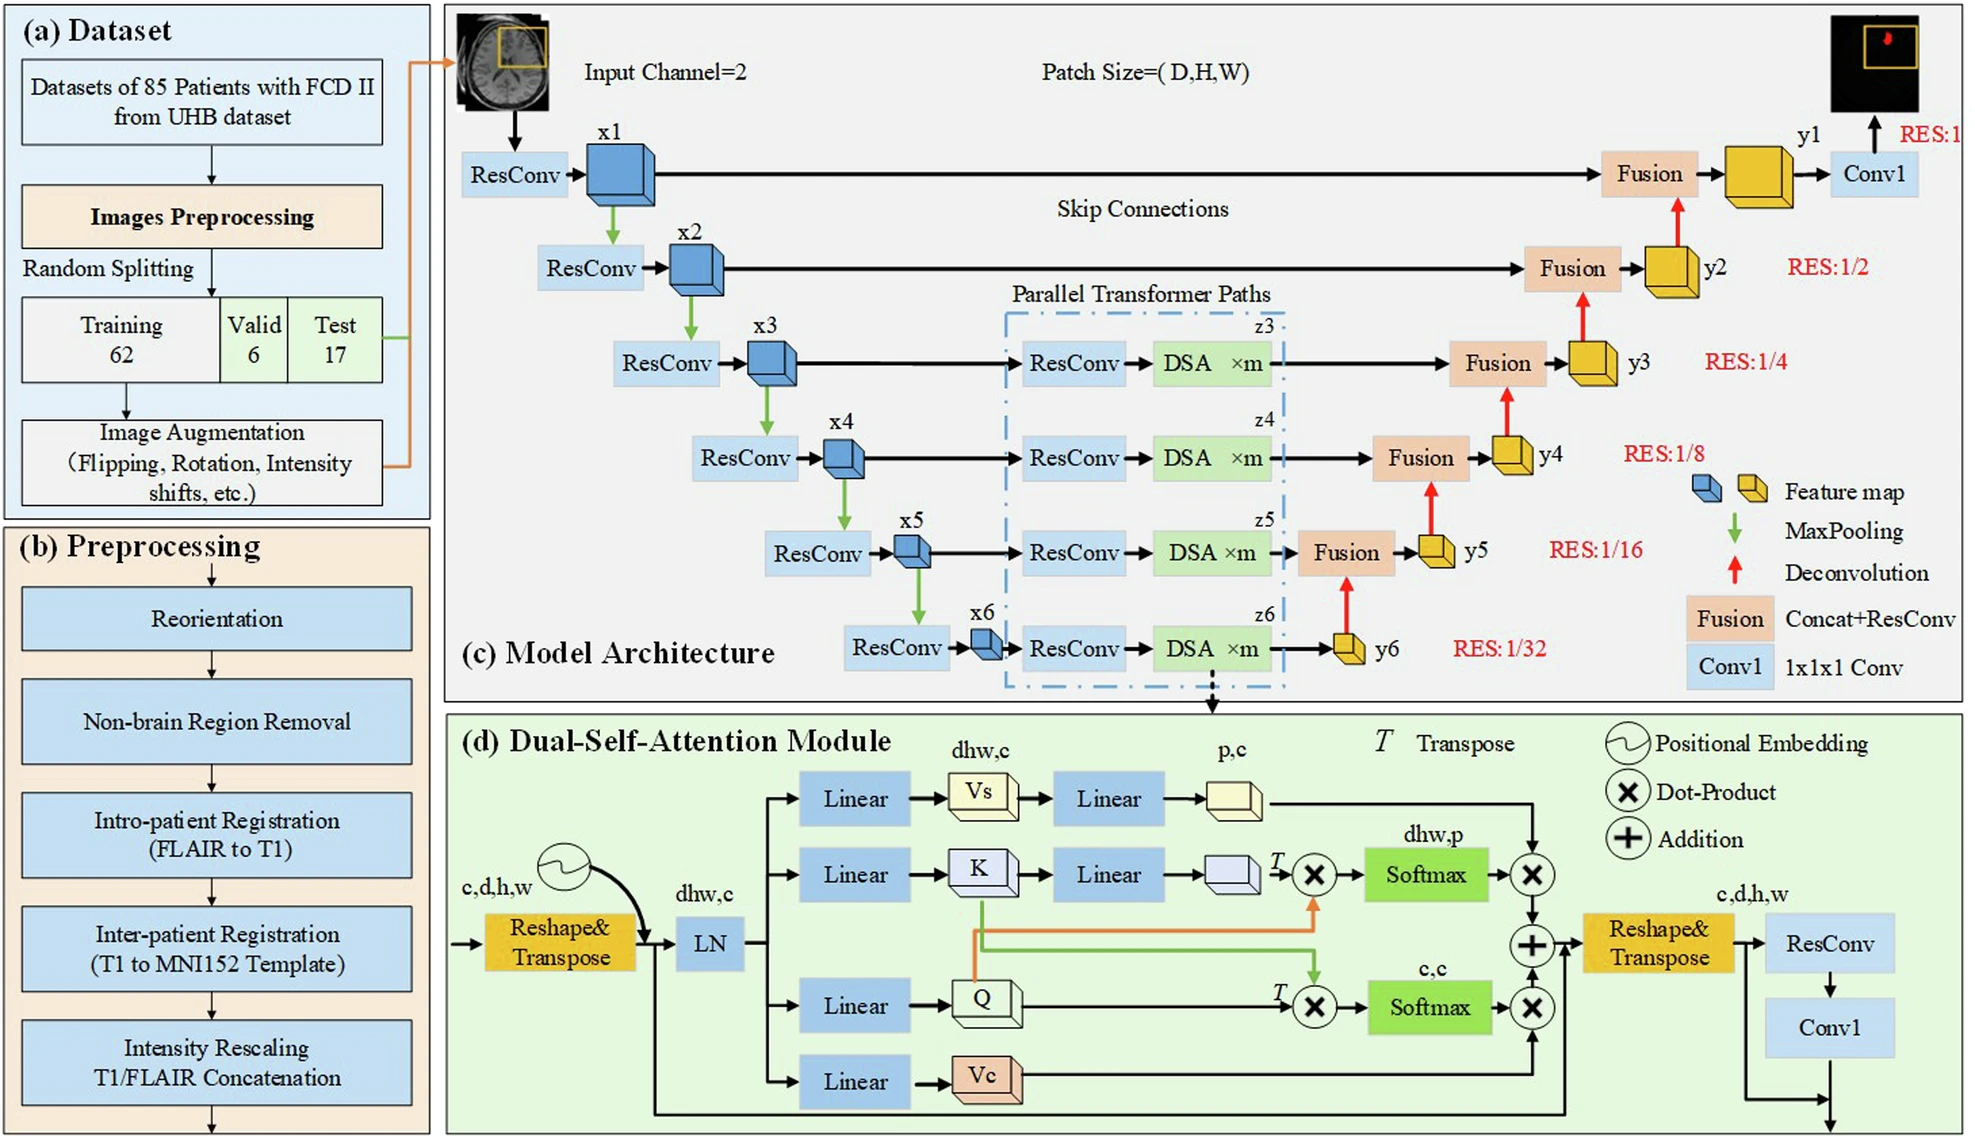
\includegraphics[width=\textwidth]{unet.png}
	\caption{a. Dataset splitting; b. Preprocessing procedure; c. Architecture of the proposed model based on an encoder-decoder structure. Parallel transformer pathways, each consisting of m dual-self-attention (DSA) modules, are inserted to capture the global features on feature maps of different resolutions, ranging from 1/4 to 1/32. d. Architecture of the DSA module, consisting of a spatial self-attention branch and a channel self-attention branch From research: \citeref{res8}}
	\label{fig:res8}
\end{figure}

\subsubsection{Results}

Here: \citeref{tab:res8}

\begin{table}[htbp]
	\centering
	\fbox{
	\begin{tabular}{l c}
		n & 170 \\
		patients & 85 \\
		controls & 85 \\
		train ratio & 0.6 \\
		test ratio & 0.25 \\
		valid ratio & 0.15 \\
	\end{tabular}
	}
	\caption{Benchmark}

	\fbox{
	\begin{tabular}{l c}
		Sensitivity & 82.4\% \\
		Specificity & ??\% \\
		Dice coefficient & 0.410
	\end{tabular}
	}
	\caption{Results from \citeref{res8}}
	\label{tab:res8}
\end{table}

\newpage
\subsection{\href{https://www.sciencedirect.com/science/article/pii/S1746809421005486}{[NIYAS2021102951] Segmentation of focal cortical dysplasia lesions from magnetic resonance images using 3D convolutional neural networks (Sept 2021) }}
\label{res9}

Mainly focused on using as less space and memory as possible

U-Net to analyse 3D MRI images to find FCD

Nice review at the beginning with lots of references

Because of class imbalance, Tversky loss used (see \citeref{fig:res9_0})

\begin{figure}[htbp]
	\centering
	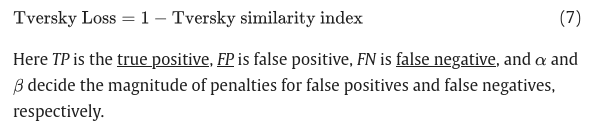
\includegraphics[width=\textwidth]{tversky_loss.png}
	\caption{From \citeref{res9}}%
	\label{fig:res9_0}
\end{figure}

\begin{figure}[htbp]
	\centering
	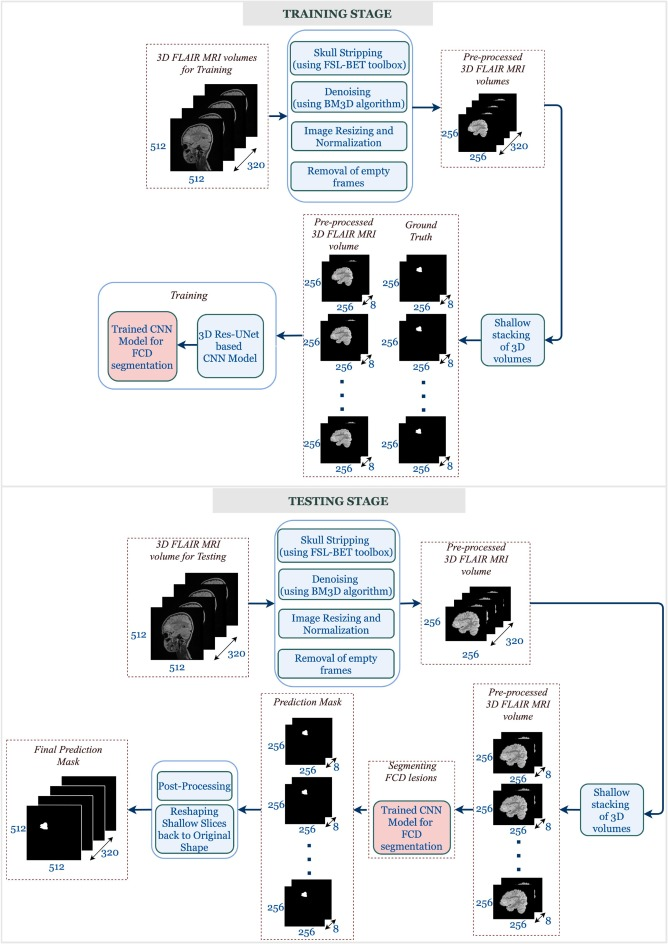
\includegraphics[width=\textwidth]{3DCNN_UNET_explanation.jpg}
	\caption{From \citeref{res9}}%
	\label{fig:res9_1}
\end{figure}

\begin{figure}[htbp]
	\centering
	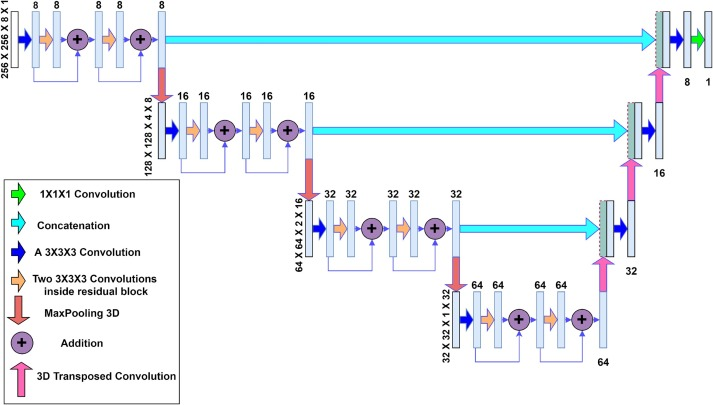
\includegraphics[width=\textwidth]{3DCNN_UNET_explanation_2.jpg}
	\caption{From \citeref{res9}}%
	\label{fig:res9_2}
\end{figure}

\subsubsection{Results}

Here: \citeref{tab:res9}

\begin{table}[htbp]
	\centering
	\fbox{
	\begin{tabular}{l c}
		n & ?? \\
		patients & 26 \\
		controls & ?? \\
		train ratio & 0.7 \\
		test ratio & 0.1 \\
		valid ratio & 0.2 \\
	\end{tabular}
	}
	\caption{Benchmark}

	\fbox{
	\begin{tabular}{l l l l}
		& Pixel-wise & Region-wise & Patient-wise\\
		Precision & 69.58 & 74.75 & irrelevant\\
		Recall & 61.86 & 78.69 & 93 \\
		Dice & 64.32 & 76.67 & irrelevant \\
	\end{tabular}
	}
	\caption{Results from \citeref{res8}}
	\label{tab:res9}
\end{table}

\newpage
\subsection{\href{https://ieeexplore.ieee.org/document/9198063}{[EDWIN9198063] Multi-Res-Attention UNet: A CNN Model for the Segmentation of Focal Cortical Dysplasia Lesions from Magnetic Resonance Images (May 2021) }}
\label{res10}

2D U-Net architecture

Dice loss and binary cross entropy function

\begin{figure}[htbp]
	\centering
	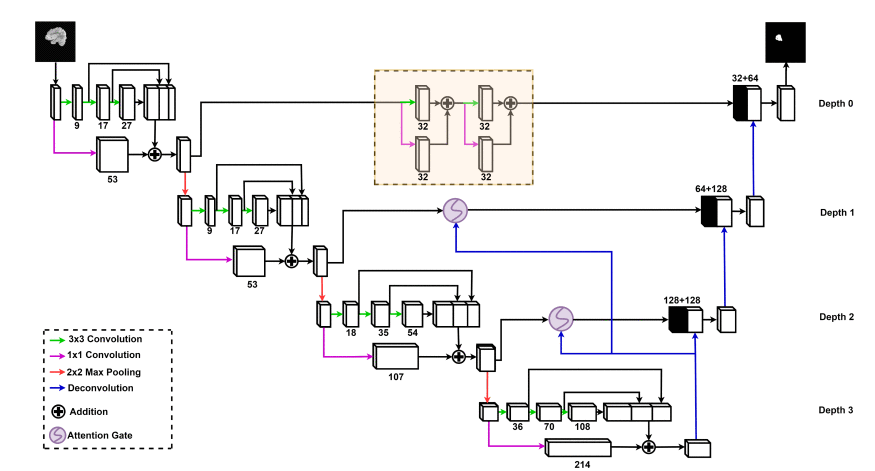
\includegraphics[width=\textwidth]{multires_attention_1.png}
	\caption{From \citeref{res10}}%
	\label{fig:res10_1}
\end{figure}
\begin{figure}[htbp]
	\centering
	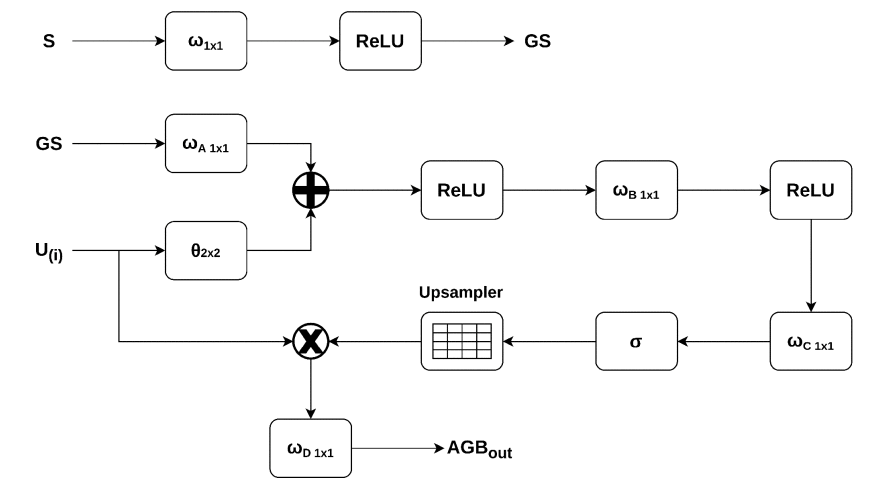
\includegraphics[width=\textwidth]{multires_attention_2.png}
	\caption{From \citeref{res10}}%
	\label{fig:res10_2}
\end{figure}

\subsubsection{Results}

Here: \citeref{tab:res10}

\begin{table}[htbp]
	\centering
	\fbox{
	\begin{tabular}{l c}
		patients & 26 \\
		train & 4302 \\
		valid & 1075 \\
		tests & 1194 \\
		train ratio & 0.7 \\
		test ratio & 0.1 \\
		valid ratio & 0.2 \\
	\end{tabular}
	}
	\caption{Benchmark}

	\fbox{
	\begin{tabular}{l l l l}
		& Pixel-wise & Region-wise & Patient-wise\\
		Precision & 68.10 & 87.97 & irrelevant\\
		Recall		& 60.23 & 67.09 & 92 \\
		Dice			& 76.62 & 76.62 & irrelevant \\
	\end{tabular}
	}
	\caption{Results from \citeref{res10}}
	\label{tab:res10}
\end{table}

\newpage
\subsection{\href{https://pmc.ncbi.nlm.nih.gov/articles/PMC10933224/}{[ZHANG202403] Deep learning-based automated lesion segmentation on pediatric focal cortical dysplasia II preoperative MRI: a reliable approach (March 2024) }}
\label{res11}

Using 3D full-resolution nnU-Net
\begin{figure}[htbp]
	\centering
	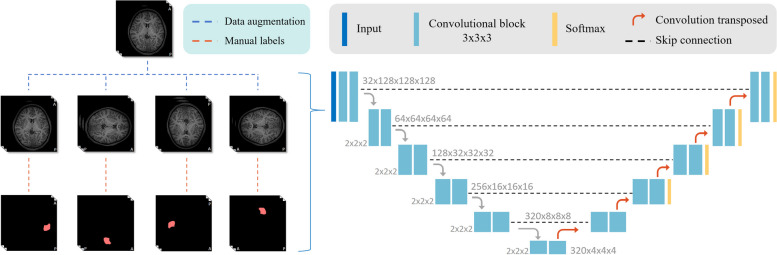
\includegraphics[width=\textwidth]{nnunet.jpg}
	\caption{From \citeref{res11}}%
	\label{fig:res11}
\end{figure}

\subsubsection{Results}

Here: \citeref{tab:res11}

\begin{table}[htbp]
	\centering
	\fbox{
	\begin{tabular}{l c}
		patients & 65 \\
		train & 200 \\
		valid & ?? \\
		tests & 15 \\
		train ratio & 0.7 \\
		test ratio & 0.1 \\
		valid ratio & 0.2 \\
	\end{tabular}
	}
	\caption{Benchmark}

	\fbox{
	\begin{tabular}{l l}
		Sensitivity & 0.73 \\
		Dice			  & 0.57 \\
	\end{tabular}
	}
	\caption{Results from \citeref{res11}}
	\label{tab:res11}
\end{table}


\newpage
\subsection{\href{https://link.springer.com/article/10.1186/s12938-020-0757-8}{[FENG202002] Detecting focal cortical dysplasia lesions from FLAIR-negative images based on cortical thickness (2020) }}
\label{res12}

Calculated a cortical thickness mean via healthy controls, then analysed patients and compared with this data

Benchmark available on demand

\begin{figure}[htbp]
	\centering
	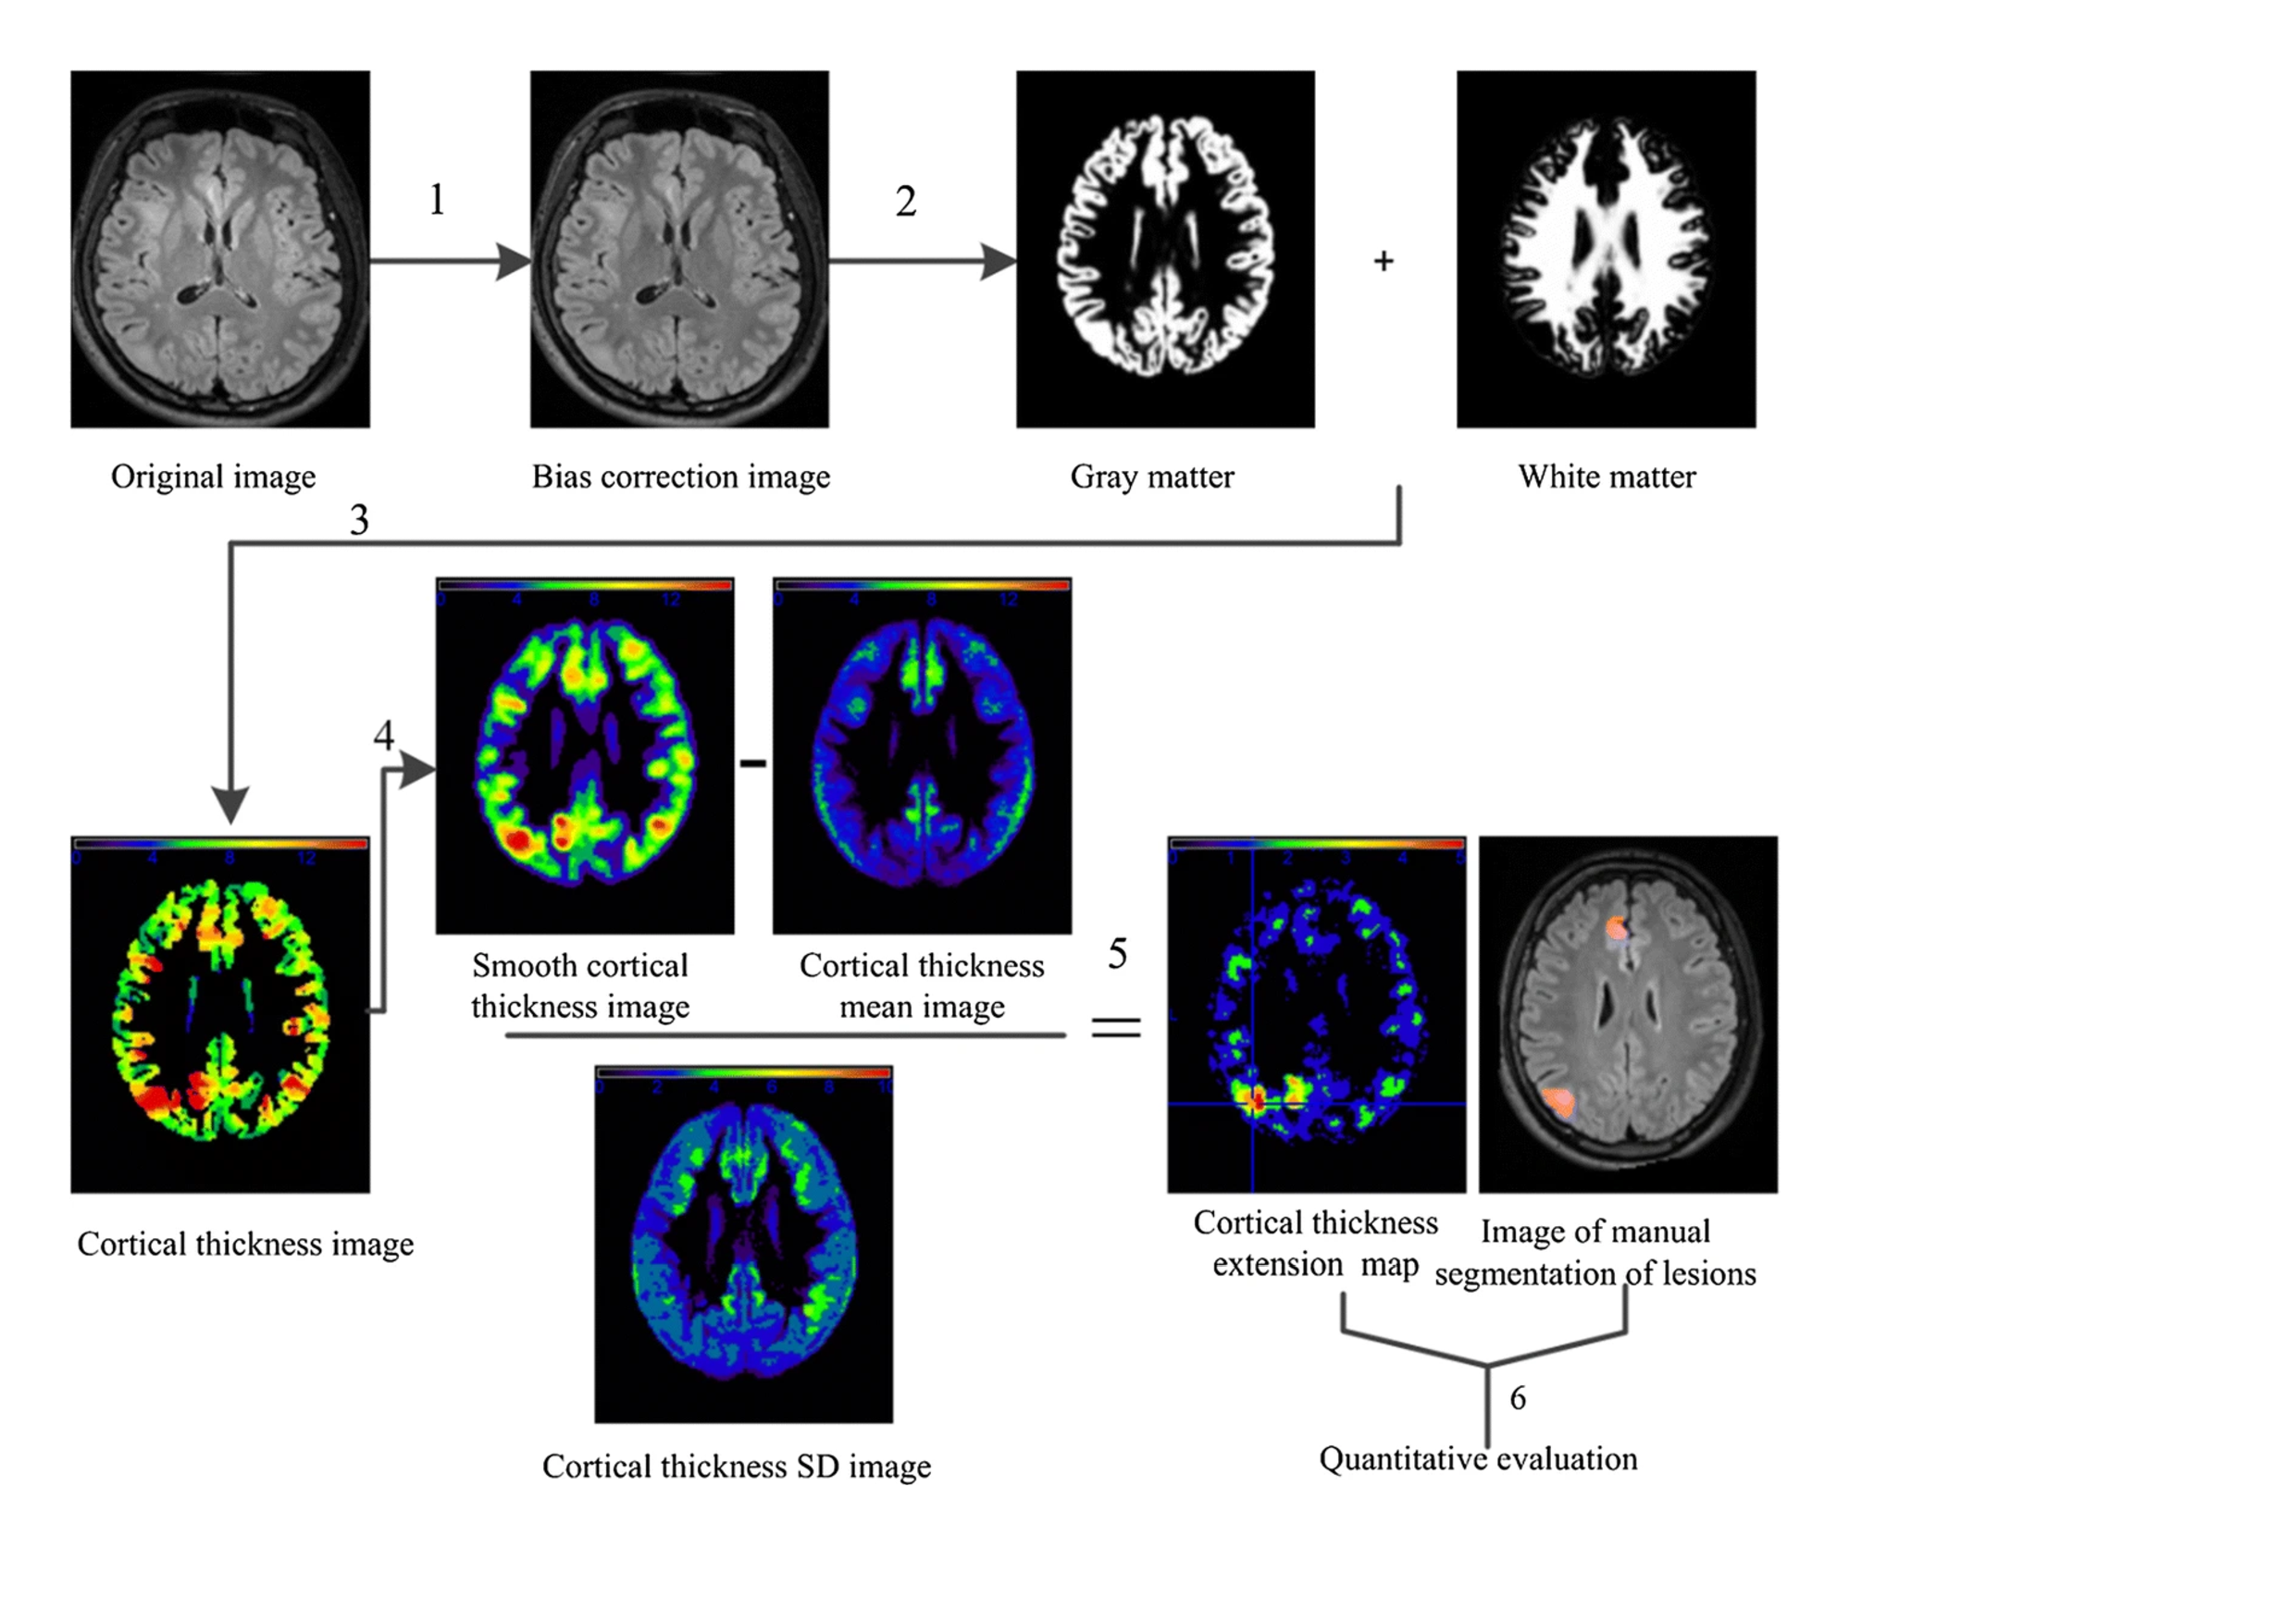
\includegraphics[width=\textwidth]{cortical_thickness_analysis.pdf}
	\caption{From \citeref{res12}}%
	\label{fig:res12}
\end{figure}

\subsubsection{Results}

Here: \citeref{tab:res12}

\begin{table}[htbp]
	\centering
	\fbox{
		\begin{tabular}{l c}
			patients & 6 \\
			controls & 32 \\
			train ratio & ?? \\
			test ratio & ?? \\
			valid ratio & ?? \\
		\end{tabular}
	}
	\caption{Benchmark}

	\fbox{
		\begin{tabular}{l l l l}
												& Voxel-wise \\
			Specificity				& 99.78			 \\
			Accuracy					& 99.76			 \\
			Recal							& 67.45			 \\
			Precision					& 20.42			 \\
			Dice							& 30.01			 \\
			Youden index			& 67.23			 \\
			Area under curve	& 83.62			 \\
		\end{tabular}
	}
	\caption{Results from \citeref{res12}}%
	\label{tab:res12}
\end{table}


\newpage
\subsection{\href{https://jamanetwork.com/journals/jamaneurology/article-abstract/2830410}{[RIPART202502] Detection of Epileptogenic Focal Cortical Dysplasia Using Graph Neural Networks (Feb 2025)}}
\label{res13}

Graph neural network to identify FCD from 3D T1 and FLAIR images

Code available here: \citeref{code:res13}

\subsubsection{Results}

Here: \citeref{tab:res13}

\begin{table}[htbp]
	\centering
	\fbox{
		\begin{tabular}{l c}
			patients & 703 \\
			controls & 482 \\
			train ratio & ?? \\
			test ratio & ?? \\
			valid ratio & ?? \\
		\end{tabular}
	}
	\caption{Benchmark}

	\fbox{
		\begin{tabular}{l l l l}
			Specificity				& 60\%			 \\
			Sensitivity				& 70\% \\
			Positive predictive value	& 67\%			 \\
		\end{tabular}
	}
	\caption{Results from \citeref{res13}}%
	\label{tab:res13}
\end{table}

\newpage
\subsection{\href{https://www.frontiersin.org/journals/human-neuroscience/articles/10.3389/fnhum.2021.608285/full}{[] Automatic Detection of Focal Cortical Dysplasia Type II in MRI: Is the Application of Surface-Based Morphometry and Machine Learning Promising? (Feb 2021)}}
\label{res14}

ANN classification

Uses morphological and intensity-based features instead of image analysis

\subsubsection{Results}

Here: \citeref{tab:res14}

\begin{table}[htbp]
	\centering
	\fbox{
		\begin{tabular}{l c}
			patients & 30 \\
			controls & 28 \\
		\end{tabular}
	}
	\caption{Benchmark}

	\fbox{
		\begin{tabular}{l l l}
												& MRI-positive & MRI-negative \\
			Specificity				& 100\%				 & -						\\
			Sensitivity				& 96.7\%			 & 91.3\% 			\\
			Accuracy					& 98.6\%			 & 91.3\%
		\end{tabular}
	}
	\caption{Results from \citeref{res14}}%
	\label{tab:res14}
\end{table}

\newpage
\subsection{\href{https://www.sciencedirect.com/science/article/pii/S1878875025003651}{[] Automated Detection and Localization of Focal Cortical Dysplasia Type II: The Optimized Detection Framework (ODF) (June 2025)}}
\label{res15}

1.5T and 3T MRI

ODF -> optimized detection framework consisting in evaluating three classification methods: artificial neural network, decision tree, and support vector machine

ANN turned out to be superior with these results: "accuracy of 98.6\%, attaining sensitivity of 97.5\% and specificity of 100\% for lesion detection. The localization accuracy for lesions was 84.2\% for hemispheric and 77.3\% for lobar classification"

\newpage
\subsection{\href{https://www.researchgate.net/publication/344780032_Convolutional_neural_networks_for_automatic_detection_of_Focal_Cortical_Dysplasia}{[] Convolutional neural networks for automatic detection of Focal Cortical Dysplasia (Oct 2020)}}
\label{res16}

Code here: \citeref{code:res16}

Classic CNN analysis

\newpage
\subsection{\href{https://www.sciencedirect.com/science/article/pii/S0895611118304610}{[] Automated detection of focal cortical dysplasia using a deep convolutional neural network (Jan 2020)}}
\label{res17}

Deep CNN

\subsubsection{Results}

Here: \citeref{tab:res17}

\begin{table}[htbp]
	\centering
	\fbox{
		\begin{tabular}{l c}
			patients & 10 \\
			controls & 20 \\
		\end{tabular}
	}
	\caption{Benchmark}

	\fbox{
		\begin{tabular}{l l}
			Specificity				& 100\%				 \\
			Sensitivity				& 90\%			 \\
		\end{tabular}
	}
	\caption{Results from \citeref{res17}}%
	\label{tab:res17}
\end{table}

\newpage
\subsection{\href{https://www.sciencedirect.com/science/article/pii/S0895611118304610}{[] Automated detection of focal cortical dysplasia using a deep convolutional neural network (Jan 2020)}}
\label{res18}

Code here: \citeref{code:res18}

Almost same benchmark here: \citeref{dt:res18}

Deep CNN with 3D T1w and T1-FLAIR on 148 patients 

\subsubsection{Methods}

\begin{figure}[htbp]
	\centering
	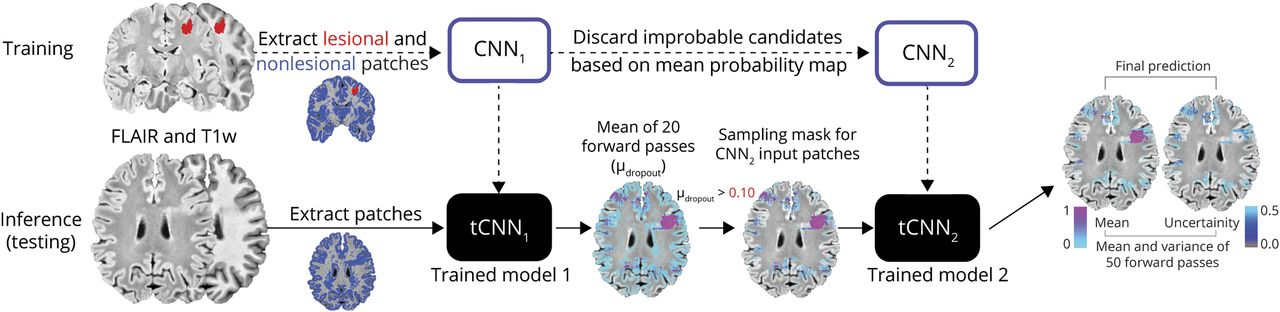
\includegraphics[width=\textwidth]{deepfcd.jpeg}
	\caption{From \citeref{res18}}%
	\label{fig:res18}
\end{figure}

\subsubsection{Results}

Here: \citeref{tab:res18}

\begin{table}[htbp]
	\centering
	\fbox{
		\begin{tabular}{l c}
			patients & 148 \\
			controls & 131 \\
		\end{tabular}
	}
	\caption{Benchmark}

	\fbox{
		\begin{tabular}{l l}
			Specificity				& 90\%				 \\
			Sensitivity				& 93\%			 \\
		\end{tabular}
	}
	\caption{Results from \citeref{res18}}%
	\label{tab:res18}
\end{table}


\newpage
\subsection{\href{https://onlinelibrary.wiley.com/doi/10.1111/epi.18240}{Detection of focal cortical dysplasia: Development and multicentric evaluation of artificial intelligence models (Dec 2024)}}

Not read

\newpage
\subsection{\href{https://pmc.ncbi.nlm.nih.gov/articles/PMC11997906/}{Detection of focal cortical dysplasia: Development and multicentric evaluation of artificial intelligence models (Dec 2024)}}

Comparison of different models with on a bigger dataset.

\newpage
\subsection{\href{https://ieeexplore.ieee.org/document/5872541}{Automated detection of Focal Cortical Dysplasia lesions on T1-weighted MRI using volume-based distributional features (March 2011)}}

Old, using image comparison rather than learning

\newpage
\subsection{\href{https://www.sciencedirect.com/science/article/pii/S1059131124000463}{Automated detection of focal cortical dysplasia based on magnetic resonance imaging and positron emission tomography (Apr 2024)}}

Using 3D Unet with T1 and PET images

Some maths for loss, and evaluation functions

\newpage
\subsection{\href{file://papers/Automatic_detection_joao.pdf}{Automatic Detection of Focal Cortical Dysplasias on Magnetic Resonance Images of Patients with Refractory Focal Epilepsy (July 2024)}}

Facts about how early epilepsy what found (2000 BCE), details about FCD Types

Work done not interesting here as it uses MELD classifier and is more about making a GUI to help clinicians.

\newpage
\section{MRI based non-supervised}
\label{ul}

\subsection{\href{https://www.sciencedirect.com/science/article/pii/S2213158220302758}{[LEE2020102438] Unsupervised machine learning reveals lesional variability in focal cortical dysplasia at mesoscopic scale (2020) }}
\label{ul1}

looking to prove that ML on MRI captures the different types of FCDs

"consensus clustering, an unsupervised learning technique that identifies stable clusters based on bootstrap-aggregation, to 3 T multicontrast MRI (T1-weighted MRI and FLAIR)"

46 patients and 46 controls

Not yet understood how it works and what is done.

\subsubsection{Results}

"Lesions were parcellated into four classes with distinct structural profiles variably expressed within and across patients: Class-1 with isolated white matter (WM) damage; Class-2 combining grey matter (GM) and WM alterations; Class-3 with isolated GM damage; Class-4 with GM-WM interface anomalies. Class membership was replicated in two independent datasets"

\newpage
\subsection{\href{https://www.sciencedirect.com/science/article/pii/S1525505015002322}{[AHMED201521] Cortical feature analysis and machine learning improves detection of “MRI-negative” focal cortical dysplasia (2015) }}
\label{ul2}

7 MRI positive, 24 MRI negative

Not sure but I believe lesions are masked on MR images before clustering.

\subsubsection{Results}

6/7 MRI positive detected and 15/24 MRI negative detected

Here: \citeref{tab:ul2}

\begin{table}[htbp]
	\centering
	\fbox{
	\begin{tabular}{l c}
		n & 93 \\
		patients & 31 \\
		controls & 62 \\
		train ratio & 0.5 \\
		test ratio & 0.5 \\
	\end{tabular}
}
	\caption{Benchmark}

	\fbox{
	\begin{tabular}{l c}
		not clear but & \\
		Sensitivity & 86\% \\
		Specificity & 58\% \\
	\end{tabular}
}
	\caption{Results from \citeref{ul2}}%
	\label{tab:ul2}
\end{table}

\newpage
\subsection{\href{https://journals.plos.org/plosone/article?id=10.1371/journal.pone.0161498}{[ELAZAMI201609] Detection of Lesions Underlying Intractable Epilepsy on T1-Weighted MRI as an Outlier Detection Problem (2016)}}
\label{ul3}

Data available: \citeref{dt:ul3}

Two methods: Statistical Parametric mapping and One-Class Support Vector Machine

Analysing two features: heteropia and blurred junction between gray and white matter

77 controls, 13 patients, 10/13 detected

\newpage
\subsection{\href{https://hal.science/tel-02062210v2/file/these.pdf}{[alaverdyan:tel-02062210] Unsupervised representation learning for anomaly detection on neuroimaging. Application to epilepsy lesion detection on brain MRI (2019)}}
\label{ul4}

Thesis on unsupervised detection. 

75 controls, 21 patients. 3D T1w and FLAIR used in both cases

Bases its work on \citeref{ul3}

\newpage
\section{EEG-based DL/ML}

\subsection{\href{https://ieeexplore.ieee.org/abstract/document/7365453}{[FUJIWARA7365453] Epileptic Seizure Prediction Based on Multivariate Statistical Process Control of Heart Rate Variability Features (2016) }}

This one uses heart rate variability because: "Because excessive neuronal activities in the preictal period of epilepsy affect the autonomic nervous systems and autonomic nervous function affects HRV, it is assumed that a seizure can be predicted through monitoring HRV."

The goal is to have real-time prediction to improve their quality of live by alerting patients of seizures and 

\newpage
\subsection{\href{https://dl.acm.org/doi/abs/10.1145/3386580}{[HUSSEIN3386580] Augmenting DL with Adversarial Training for Robust Prediction of Epilepsy Seizures (2020) }}

Using EEG, it wants to have real-time prediction. Paper not available freely.

\newpage
\section{Hippocampal sclerosis detection}
\label{hs}

\subsection{\href{https://onlinelibrary.wiley.com/doi/full/10.1002/ana.27089}{Automated and Interpretable Detection of Hippocampal Sclerosis in Temporal Lobe Epilepsy: AID-HS (Nov 2024)}}
\label{hs1}

Code here: \citeref{code:hs1}

\insertfigure{aid-hs.jpg}{hs1}
